\documentclass[11pt]{article}
\usepackage[T1]{fontenc}
\usepackage[utf8]{inputenc}
\usepackage{lmodern,microtype,amsmath,amssymb,amsthm,mathtools}
\usepackage[a4paper,margin=28mm]{geometry}
\usepackage{xcolor,xurl,enumitem,booktabs,tikz}
\usetikzlibrary{arrows.meta,calc}
\usepackage[unicode,colorlinks=true,linkcolor=blue!45!black,
 citecolor=green!35!black,urlcolor=blue!55!black]{hyperref}
\setlength{\emergencystretch}{2em}
\numberwithin{equation}{section}
\newtheorem{theorem}{Theorem}[section]
\newtheorem{proposition}[theorem]{Proposition}
\newtheorem{lemma}[theorem]{Lemma}
\newtheorem{corollary}[theorem]{Corollary}
\theoremstyle{definition}
\newtheorem{definition}[theorem]{Definition}
\theoremstyle{remark}
\newtheorem{remark}[theorem]{Remark}
\newcommand{\ii}{\mathrm i}
\newcommand{\Rea}{\operatorname{Re}}
\newcommand{\Ima}{\operatorname{Im}}
\newcommand{\Vol}{\operatorname{Vol}}
\newcommand{\Log}{\operatorname{Log}}
\title{Circle patterns and primitive fillings of augmented links}
\author{}
\date{}
\begin{document}
\maketitle
\begin{abstract}
A simple triangulated sphere with a matching of its dual determines a
link diagram with specified crossing circles. We construct the complete
hyperbolic exterior, deform one common marked circle pattern, and
calculate the original peripheral words. An explicitly normalized
classical action then has a critical point for all independently
sufficiently long signed fillings. Its real critical value, multiplied
by \(2\pi\), is the volume of the smoothly filled original exterior.
The proof includes the logarithmic torus periods and the absolute
fundamental-chain comparison; an exponentiated filling equation alone
would not imply either conclusion. No quantum asymptotic is used.
The final section states the precise interface with the separate
oscillatory filling theorem.
\end{abstract}

\section{The diagram, the action, and the theorem}

An \emph{augmented diagram} consists of strands in a projection sphere,
with disjoint two-strand crossing boxes. Around each box is an auxiliary
unknotted component, its \emph{crossing circle}, bounding a disk pierced
twice by the strands. Removing full twists leaves either no crossing
or one signed half twist in each box. The disk and its collar are
retained: they specify the peripheral curves used to put the full
twists back.

Here is the combinatorial input throughout this paper. Let
\(\mathcal T\) be a finite oriented simple triangulated sphere with
at least four vertices. Choose a perfect matching of its cubic dual.
Two matched triangles share one edge and have distinct third vertices.
Write their cyclic quadrilateral as
\((x_e,b_e,y_e,c_e)\); its diagonal is \(x_ey_e\).
The triangles are the input \((x_e,b_e,y_e)\) and output
\((x_e,c_e,y_e)\), with their sphere orientations understood.
There are \(R\) matched pairs and \(R+2\) white vertices.
An edge of \(\mathcal T\) whose dual is not in the matching will be
called a \emph{strand edge}. Choose such an edge \(uv\) as a mark.

The inverse cut in Section~\ref{mf:topology} constructs from these data
an augmented link in \(S^3\). Equivalently, the input may be an actual
augmented diagram whose projection and disk cut has exactly these
labels and orders. At each disk retain
\(\epsilon_e\in\{-1,0,1\}\) half twists, with the positive convention
specified by the Hurwitz move in \eqref{mf:hurwitz}. Denote the resulting
augmented exterior by \(Y_D\). Its main components are the original
strands; its auxiliary components are the crossing circles.

On each auxiliary cusp choose the original disk-framed primitive
meridian and longitude \((\mu_e,\lambda_e)\). The meridian goes once
around the crossing circle. The longitude follows its twice-punctured
disk and is represented by the ordered product \(P_e=B_eA_e\) of the
two based main meridians. The orientation and basepaths will be checked
in Section~\ref{mf:words}. Filling the slope
\(\mu_e+p_e\lambda_e\), \(p_e\in\mathbb Z\), inserts \(-2p_e\)
crossings, so the restored power is
\begin{equation}\label{mf:powers}
                         n_e=\epsilon_e-2p_e.
\end{equation}
The original outside pairing and these box parities determine the main
components. We call the filled link a knot only when that terminal
graph is connected.

We use curvatures, not radii, as the variables of the action. A finite
white circle with curvature \(w>0\) has radius \(1/w\). The two marked
white circles will be parallel lines and have curvature zero.
For three nonnegative curvatures, not all zero, define
\begin{equation}\label{mf:triangle}
\begin{split}
 F(w_1,w_2,w_3)
 &=\frac1{2\pi}
  \max_{\substack{\theta_j\ge0\\\sum_j\theta_j=\pi}}
      \left\{\sum_j\theta_j\log w_j+\mathcal V(\theta)\right\},\\
 \mathcal V(\theta)
 &=2\sum_{j=1}^3
   \left[\Lambda(\theta_j/2)+
                 \Lambda((\pi-\theta_j)/2)\right],\\
 \Lambda(t)&=-\int_0^t\log|2\sin s|\,ds.
\end{split}
\end{equation}
A zero curvature forces its angle to zero; its logarithmic term is
omitted. Thus \(F(w,0,0)=\frac12\log w\). This definition fixes the
absolute constant geometrically.

For one triangle \((x,b,y)\), introduce a small complex parameter
\(\delta\), and put
\begin{equation}\label{mf:local-data}
\begin{aligned}
 s&=\sin(\pi\delta),& c_0&=\cos(\pi\delta),& A&=x+y,\\
 D&=A^2-4xy s^2,&
 T_b&=\sqrt{bA+xy+b^2s^2},&
 E_b&=A+2bs^2+2sT_b.
\end{aligned}
\end{equation}
The square roots are continued from positive complete values. In a
singleton triangle, where a middle and an outer curvature are zero,
set \(T_b=0\) and \(E_b=A\) exactly. At every matched pair \(A>0\).
Define the holomorphic triangle germ \(Q_b\) by
\begin{equation}\label{mf:Q}
 Q_b(0;x,b,y)=F(x,b,y),\qquad
 \partial_\delta Q_b=-\Log(E_b/\sqrt D),
\end{equation}
with logarithm zero at \(\delta=0\). Section~\ref{mf:pattern} proves
that it is an angle potential for the deformed common pattern.
It has logarithmic homogeneity \(1/2\), as does \(F\).

Set \(w_u=w_v=0\), fix one common scale of the ordinary curvatures,
and define the selected face-critical value
\begin{equation}\label{mf:A0}
 A_0(\boldsymbol\delta)
   =\operatorname{crit}_{w}
       \left\{\sum_{e=1}^R(Q_{b_e}+Q_{c_e})
                       -\sum_{f\ne u,v}\Log w_f\right\}.
\end{equation}
The critical point in this definition is the unique germ at the
complete positive packing. Its existence is proved below.

\begin{theorem}[Primitive fillings and their classical action]
\label{mf:main}
For every fixed marked matched sphere and its retained signed collars,
the action \eqref{mf:A0} is holomorphic near zero, separately even,
and real on real parameters. Its complete value is
\[
             A_0(0)=\Phi_D=\frac{\Vol(Y_D)}{2\pi}.
\]
There is a diagram-dependent threshold \(T_D\) with the following
property. For every fixed integer vector \(\mathbf p\) with
\(\min_e|n_e|>T_D\), the function
\begin{equation}\label{mf:filling-action}
 S_{\mathbf n}(\delta)=A_0(\delta)+
       \pi\ii\sum_e n_e\delta_e^2+2\pi\ii\sum_e\delta_e
\end{equation}
has one critical point in the selected small germ. At that point:
\begin{enumerate}[label=(\roman*)]
\item The explicitly constructed representation of \(\pi_1(Y_D)\)
has original primitive similarity logarithms
\begin{equation}\label{mf:logs}
 U_e=-\Log(E_{b_e}E_{c_e}/D_e)+2\pi\ii\epsilon_e\delta_e,
 \qquad V_e=-4\pi\ii\delta_e,\qquad
 U_e+p_eV_e=-2\pi\ii .
\end{equation}
Moreover \(\Ima\delta_e>0\), for either sign of \(n_e\).
\item It is the holonomy of a smooth complete finite-volume hyperbolic
metric on the original filled exterior
\(Y_D(\mu_e+p_e\lambda_e)_e\). Every main cusp remains complete.
\item Its critical value satisfies the absolute equality
\begin{equation}\label{mf:volume}
 2\pi\Rea S_{\mathbf n}
       =\Vol\bigl(Y_D(\mu_e+p_e\lambda_e)_e\bigr).
\end{equation}
\end{enumerate}
If the original component test is a knot, the right side is
\(\Vol(S^3\setminus K_{\mathbf p})\).
As all \(|n_e|\) tend to infinity, the critical point tends to zero
and \(\Rea S_{\mathbf n}\to\Phi_D\).
\end{theorem}

The sphere, its matching, collars and filling integers are fixed before
any asymptotic application. The threshold places no restriction on the
ratios or signs of the independently long powers. The uniqueness claim
concerns the indicated critical germ; it is not uniqueness of the whole
character variety. No quantum limit occurs in the theorem.

Variational existence and uniqueness for circle patterns, and their
relation to hyperbolic volume, are classical;
see Rivin~\cite{Rivin} and Bobenko--Springborn~\cite{BobenkoSpringborn}.
We give the particular
packing and deformation arguments needed here, including the marked
lines and the original peripheral paths. We use the elementary
holomorphic implicit-function theorem, differential forms and Stokes;
for the smooth background see~\cite[Chapters 4 and 16]{Lee}.
The implicit-function arguments may equivalently be obtained by
preconditioning the equation with its invertible linear part and
applying uniform contraction on a small complex ball. The resulting
fixed point is holomorphic as the locally uniform limit of its
holomorphic iterates.
The ideal-tetrahedron volume formula used below is the classical
Lobachevsky formula; see~\cite[Appendix]{Milnor}. We prove the global
normalizations and filling comparison rather than importing a general
Dehn filling or character-rigidity theorem.

\section{A packing and the original complete exterior}\label{mf:topology}

\subsection{Strict feasibility and the circle packing}

\begin{proposition}[Packing with its exact labels]\label{mf:packing}
Every simple triangulated sphere in the hypotheses has a packing of
white disks, with contacts exactly its edges. The circles through the
three contacts of each triangular interstice bound orthogonal shaded
planes. These planes and the white planes bound a convex ideal
right-angled polyhedron with precisely the prescribed medial sphere.
\end{proposition}
\begin{proof}
Remove a triangular face \(abc\), and prescribe positive boundary
radii \(r_a,r_b,r_c\). The remaining disk, with \(v\) interior
vertices, has \(2v+1\) triangles by Euler's formula.
Give each triangle angle supply \(\pi\), each interior vertex demand
\(2\pi\), and the three boundary vertices pooled demand \(\pi\);
their separate corners are retained.

We first find a strictly positive allocation to all corners.
A nonempty set \(S\) of interior vertices touches at least
\(2|S|+1\) disk triangles. Indeed, puncture the sphere at a vertex
of \(S\). On the complementary interior vertices \(T\) and \(a,b,c\),
a simple planar graph has at most \(2|T|+1\) bounded triangular
faces. One is the omitted face \(abc\), so at most \(2|T|\) disk
triangles avoid \(S\). A proper destination set containing the pooled
boundary destination also has strict slack: its complement \(T\)
consists only of interior vertices, and at most \(2|T|-5\) triangles
are wholly supported there for \(|T|\ge3\), with none for
\(|T|\le2\). The full destination set has equal demand and supply.

These are the finite transport Hall inequalities. To recall the short
argument, join a source to the triangle nodes with their supply
capacities, join each triangle to its incident destinations, and join
destinations to a sink with their demands. A finite cut minimizes to
one of these inequalities. Augmenting along residual paths proves
feasibility for rational capacities; compactness gives the real case.
Strict slack at every proper destination subset permits subtraction
of one small positive amount at every corner before this argument.
Thus an allocation positive at every corner exists.

On the compact angle polytope maximize
\[
       \sum_t\mathcal V(\theta_t)
          +\sum_{\text{boundary corners }tf}\theta_{tf}\log(1/r_f).
\]
For \(0<\theta<\pi\), the corner derivative of \(\mathcal V\) is
\(-\log\tan(\theta/2)\), and its second derivative is
\(-1/\sin\theta<0\). A maximum is interior: moving toward the
strictly positive allocation gives a positive
\(\varepsilon\log(1/\varepsilon)\) contribution at each new zero
corner, a nonnegative one at an old \(\pi\) corner, and only bounded
linear costs elsewhere. Strict feasibility alone would not establish
this boundary exclusion. Strict concavity now makes the maximum unique.
Its Lagrange multipliers give positive curvatures \(w_f=1/r_f\),
including the prescribed boundary ones, and
\begin{equation}\label{mf:angles}
 \tan(\theta_{tf}/2)=\frac{w_f}{D_t},\qquad
 D_t=\sqrt{\sum_{\{f,g\}\subset t}w_fw_g}.
\end{equation}
The row sum \(\pi\) determines \(D_t\) by the tangent addition
identity. These are the angles of the Euclidean center triangle
with sides \(r_f+r_g\).

Glue those center triangles. Interior angle sums are \(2\pi\).
Continuation around an interior vertex fixes that vertex and rotates
by \(2\pi\), hence has zero translation as well as rotation.
Such loops generate the punctured disk's holonomy, so the development
is globally defined. Its boundary consists of the three prescribed
straight sides; each boundary angle sum is positive and less than
\(\pi\), and their total is \(\pi\). It therefore traverses a convex
triangle once. The development is locally orientation-preserving at
every interior point. For a point off the developed edges the number
of preimages is its boundary winding number, one inside and zero
outside. Local injectivity extends the conclusion across the edges
and vertices. Thus the development is an embedding.

Place each radius-\(r_f\) disk at its developed center. In a center
triangle the opposite edge is covered by the other two tangent disks,
both disjoint from the third. Their mutual contact is strictly outside
the third disk, whose contacts with them lie on the two incident edges.
Consequently the third disk's sector stops strictly before the opposite
edge. Sectors assemble to full disks at interior vertices and to the
prescribed boundary sectors. This proves disjoint interiors and
excludes unintended contacts, even across separating triangles.

The circle through a triangle's three contacts is its incircle:
the contact distance along a center edge is the corresponding radius.
It is orthogonal to each vertex circle. Its disk lies in its center
triangle and contains no other packing contact. For the omitted outer
triangle choose the opposite side of its contact circle; all interior
contacts lie in its bounded curvilinear gap and therefore inside that
circle. Each contact consequently lies in all prescribed inward white
and shaded halfspaces, strictly unless incident. The exposed faces
form the closed labeled medial sphere, so the convex hull has exactly
those facets. Four faces alternate at every contact, with successive
right angles. This constructs the stated polyhedron \(Q\).
\end{proof}

Sending the contact of the marked edge \(uv\) to infinity by one
orientation-preserving Möbius map makes its white disks the outward
halfplanes \(Y\le0\) and \(Y\ge1\). All other disks are bounded in the
strip. The curvature scale is immaterial. In particular exactly the
two marked curvatures vanish.

\subsection{The reversible cut and primitive cusps}

Take disjoint small disk neighborhoods of the matched dual edges.
They are four-terminal disks. At disk \(e\), write the cyclic
terminals \(C_0,C_1,C_2,C_3\). The two shaded halves group
\((C_1,C_2)\) and \((C_3,C_0)\), while the untwisted physical
strands join \((C_0,C_1)\) and \((C_2,C_3)\).
Join the outside terminals along the nonmatching dual edges, and
place a perpendicular crossing circle and its disk in each disjoint
three-ball collar. This is an embedded link in \(S^3\).
For odd parity the physical pairing is
\((C_0,C_2),(C_1,C_3)\).
The outside and inside terminal matchings form a degree-two graph;
its connectedness is exactly the knot test. Full twists do not change it.

Cut the augmented exterior along the projection sphere. In each
projection ball every crossing-circle semicircle is boundary parallel
by its original half disk. Drilling that semicircle and opening that
same half disk cancels the introduced handle. The half disks are
disjoint, so all these operations leave a ball in each copy.
Its boundary is the labeled medial sphere of Proposition~\ref{mf:packing}.
The boundary cell identification with \(Q\) extends radially over
the ball. Cycles in the matching graph introduce no extra handle.

Use two copies \(Q^+,Q^-\). White faces glue across copies by their
projection labels. At an even disk, in each copy, the shaded pairing fixes
the crossing-circle vertex \(O_e\) and sends
\begin{equation}\label{mf:even-corners}
                   C_1\longmapsto C_0,\qquad C_2\longmapsto C_3.
\end{equation}
At an odd disk it interchanges copies and punctures:
\begin{equation}\label{mf:odd-corners}
\begin{aligned}
 (O,C_1,C_2)^+&\longmapsto(O,C_3,C_0)^-,\\
 (O,C_3,C_0)^+&\longmapsto(O,C_1,C_2)^- .
\end{aligned}
\end{equation}
These maps follow by rotating one side of the twice-punctured disk
by \(\pm\pi\), which sends its normal coordinates \((y,z)\) to
\((-y,-z)\). The two signs have the same corner permutation but
different collar paths. Those paths will remain in the peripheral
calculation.

Every ideal vertex link of \(Q\) is a rectangle. Choose its horosphere
so its two opposite shaded sides have length one. Thus every shaded
ideal triangle has its canonical length-one horocycles at its three
corners. The prescribed triangle maps, including odd permutations,
preserve them, as do the white identifications. Each edge cycle has
four pieces and angle \(2\pi\). It fixes the two ideal endpoints,
preserves both horospheres, and therefore has zero translation along
the edge as well as rotation \(2\pi\); its full holonomy is the identity.
The links glue to the original torus links without cone or dilation
defects. Their horoball ends are complete, and the remaining part is
compact. We have proved
\begin{equation}\label{mf:complete-volume}
                         \Vol(Y_D)=2\Vol(Q).
\end{equation}

This quotient also has a positive ideal triangulation. Choose a vertex
of \(Q\), triangulate its nonincident faces, and cone their triangles
to that vertex; fan the incident faces. Strict support makes every
tetrahedron nondegenerate and positive. Use identical white
subdivisions in the two copies; shaded faces were already triangles.
These are cells of this exterior, not an assumed triangulation of a
later filled manifold.

\subsection{The absolute complete action}

At the complete marked packing, let \(\theta_{tf}\) be the center
angles, with the usual line limits. A singleton triangle has angles
\((\pi,0,0)\). Formula \eqref{mf:angles} and strict concavity prove
\[
 2\pi F(w_t)=\mathcal V(\theta_t)+\sum_{f\in t}\theta_{tf}\log w_f,
 \qquad \partial_{\log w_f}F=\theta_{tf}/(2\pi).
\]
The finite-circle angle sums are \(2\pi\), so the complete packing
is stationary for
\(\sum_tF(w_t)-\sum_{f\ne u,v}\log w_f\).

To fix its absolute value, cone the marked ideal vertex, now infinity,
to every nonincident facet of \(Q\). These positive pyramids partition
\(Q\). For a cyclic white ideal polygon with consecutive central
arcs \(\alpha_j\), its cone volume is
\(\sum_j\Lambda(\alpha_j/2)\). Triangulate the polygon: the ideal
tetrahedron formula gives three Lobachevsky values, and internal
diagonal half-arcs cancel by \(\Lambda(\pi-t)=-\Lambda(t)\).
At a shaded triangle the white contact arcs are \(\theta_{tf}\).
Orthogonality gives complementary shaded arcs \(\pi-\theta_{tf}\).
Consequently
\[
 \Vol(Q)=\sum_{t,f\in t}
  \left[\Lambda(\theta_{tf}/2)+
                  \Lambda((\pi-\theta_{tf})/2)\right]
                =\frac12\sum_t\mathcal V(\theta_t).
\]
Incident line facets and singleton triangles contribute zero by
continuity. Canceling the angle-weight terms against the original
face targets proves
\begin{equation}\label{mf:Phi}
 \Phi_D=\sum_tF(w_t)-\sum_{f\ne u,v}\log w_f
                    =\Vol(Q)/\pi=\Vol(Y_D)/(2\pi).
\end{equation}
The constant \(F(w,0,0)=\frac12\log w\) is essential here.

\section{One holomorphic marked pattern}\label{mf:pattern}

Use the strip \(0<Y<1\). For each ordinary circle retain its center
\((X_f,Y_f)\) and radius \(r_f\). A strand edge has inversive cosine
\(I_{fg}=1\), and a matching edge \(e\) has
\(I_{fg}=\cos(2\pi\delta_e)\). The actual signed equations are
\begin{equation}\label{mf:circle-system}
\begin{aligned}
 (X_f-X_g)^2+(Y_f-Y_g)^2
          &=r_f^2+r_g^2+2I_{fg}r_fr_g,\\
 Y_f&=r_f I_{uf} &&\text{on the lower line},\\
 1-Y_f&=r_f I_{vf} &&\text{on the upper line}.
\end{aligned}
\end{equation}
The line-line edge is automatic. Fix one finite center's \(X\)
coordinate. There are \(3R-1\) equations and \(3R-1\) variables.
Complexification treats \(X,Y,r\) as independent holomorphic coordinates;
it does not conjugate the deformation parameters.

\begin{lemma}[The complete pattern Jacobian]\label{mf:pattern-rank}
The Jacobian of \eqref{mf:circle-system} in these normalized variables
is invertible at completeness.
\end{lemma}
\begin{proof}
For the ordinary corners \(I_t\) of one triangle put
\(q_i=\log w_i\), \(D_t^2=\sum_{i<j}w_iw_j\).
Direct differentiation of \eqref{mf:angles} gives
\begin{equation}\label{mf:hessian}
\begin{aligned}
 \partial_{q_i}F_t&=\pi^{-1}\arctan(w_i/D_t),\\
 \partial_{q_iq_j}F_t&=-\kappa^t_{ij},\qquad
 \kappa^t_{ij}=\frac{w_iw_j}{2\pi D_t(w_i+w_j)}>0\quad(i\ne j),\\
 h^{\mathsf T}\nabla^2F_t h
      &=\sum_{i<j}\kappa^t_{ij}(h_i-h_j)^2 .
\end{aligned}
\end{equation}
For three corners use
\(D_t^2+w_i^2=(w_i+w_j)(w_i+w_k)\); two corners are its
zero-curvature limit. Homogeneity gives zero row sums. A singleton
has potential \(q_i/2\) and zero Hessian.

Deleting \(u,v\) leaves a connected ordinary graph. Reroute any path
through \(u\) along its cyclic link; then reroute through \(v\)
along its link with \(u\) removed, which is a connected path.
Every surviving edge contributes positive conductance in
\eqref{mf:hessian}. Hence the full Hessian has precisely the
constant kernel.

An infinitesimal solution of the circle equations preserves the
cyclic order of the center directions. Their angle sums at finite centers remain
\(2\pi\), so the Hessian calculation makes every logarithmic radius
variation the same scale. The two triangles containing \(uv\)
have a circle tangent to both lines. Its complete radius is \(1/2\);
linearizing its two line equations gives \(dr=0\).
Thus every radius variation is zero.

With radii fixed, each finite center triangle has one infinitesimal
Euclidean motion. A one-line triangle has \(dY_f=dY_g=0\);
its horizontal separation is \(2\sqrt{r_fr_g}>0\), and its fixed
edge gives \(dX_f=dX_g\). Its motion is horizontal translation.
Delete the two triangles incident to \(uv\). The remaining
triangulated disk has connected triangle adjacency, contains every
finite vertex, and contains a one-line triangle. Across a finite
edge, agreement at two distinct centers identifies the motions.
Across a line edge, agreement at the common finite center identifies
the two horizontal translations. All centers therefore have the same
horizontal translation. The fixed \(X\) coordinate removes it.
The square Jacobian has zero kernel.
\end{proof}

The holomorphic implicit-function theorem now gives a unique nearby
pattern on one fixed polydisk. It is real for real parameters and even
separately in each \(\delta_e\). Radii stay nonzero. Real cyclic
orders and main tangencies persist.

We identify its angle potential explicitly. For one deformed triangle,
the middle and outer angles satisfy
\begin{equation}\label{mf:deformed-angles}
\begin{aligned}
 \theta_b&=2\arctan(bc_0/T_b),\\
 \cos\theta_x&=
  \frac{x(y-x)+b(y+x\cos(2\pi\delta))}{(x+b)\sqrt D},\\
 \sin\theta_x&=\frac{2xc_0T_b}{(x+b)\sqrt D}.
\end{aligned}
\end{equation}
Exchange \(x,y\) for the third angle. Differentiation gives
\[
 \partial_\delta(\theta_f/(2\pi))
              =-\partial_{\log w_f}\Log(E_b/\sqrt D).
\]
For the middle angle both sides are \(-bs/T_b\). For an outer
angle, differentiate its sine and cosine and use their squared sum
one; substitution gives the same identity. At zero the derivatives
are those of \(F\), so integration with \eqref{mf:Q} proves
\begin{equation}\label{mf:angle-gradient}
                   \partial_{\log w_f}Q_b=\theta_f/(2\pi).
\end{equation}
One zero curvature is the line limit. With two zero curvatures the
only finite angle is \(\pi\), and the potential is \(\frac12\log w\).

The common pattern's angle sums prove the face-critical equations.
The grounded Hessian \eqref{mf:hessian} gives their unique normalized
holomorphic solution, so it is exactly the germ used in \eqref{mf:A0}.
In particular, the two degenerate triangles at the mark do not choose
their strip widths independently: a finite circle tangent to one line
and with inversive angle \(2\pi\delta_e\) at the other obeys
\begin{equation}\label{mf:strip}
                    r_f(1+\cos(2\pi\delta_e))=1.
\end{equation}
The circle equations, rather than a repeated scalar root, enforce this
common strip.

The ordered product of outer reflections has trace
\(-2\cos(2\pi\delta_e)\). Its noncentral complete parabolic limit
has a unit off-diagonal entry in some chart. The eigenvalues
\(J_e=-e^{-2\pi\ii\delta_e}\) and \(J_e^{-1}\) therefore specify
holomorphic fixed-line germs: solve the linear eigenvector equation
using that unit entry. The two flags may coincide at completeness;
no division by their difference is needed.

\section{The crossing disk and the original peripheral words}
\label{mf:words}

\subsection{One primitive sidepairing}

We calculate a map, not just its multiplier. Products act from right
to left. Let \(\mathcal R_f\) denote reflection in white circle \(f\).
The ordered input and output main meridians are
\begin{equation}\label{mf:ordered-pairs}
\begin{aligned}
 A_{\rm in}&=\mathcal R_b\mathcal R_x,&
 B_{\rm in}&=\mathcal R_y\mathcal R_b,&
 P&=B_{\rm in}A_{\rm in}=\mathcal R_y\mathcal R_x,\\
 A_{\rm out}&=\mathcal R_c\mathcal R_x,&
 B_{\rm out}&=\mathcal R_y\mathcal R_c.
\end{aligned}
\end{equation}
The actual contacts are \(C_1=x\cap b,\ C_2=b\cap y\) and
\(C_0=x\cap c,\ C_3=c\cap y\). The pure disk pairs
\(C_1\mapsto C_0,\ C_2\mapsto C_3\).

First take positive finite curvatures and small real \(\delta>0\).
Place the outer centers at \(0,L\), where
\[
 L^2=(r_x+r_y)^2-4r_xr_y s^2=\frac{D}{x^2y^2}.
\]
Their intersections are \(P_\pm=u\pm\ii v\), with
\[
 u=\frac{L^2+r_x^2-r_y^2}{2L},\qquad
 v=\frac{2sc_0}{\sqrt D}.
\]
The input middle center lies above the outer center line, the output
below it. Their coordinates are
\[
 p_f=u+\frac{r_f(r_x-r_y)}L,\qquad
 q_b=\frac{2c_0T_b}{b\sqrt D},\qquad
 q_c=-\frac{2c_0T_c}{c\sqrt D}.
\]
Subtracting the three orthogonality equations shows that the shaded
circle on side \(b\) has center \(u+\ii t_b\), where
\[
 t_b=\frac{c_0(A+2bs^2)}{\sqrt D\,T_b},
 \qquad \text{squared radius }t_b^2-v^2.
\]
On side \(c\) the analogous center has negative imaginary part.
In the coordinate \(w=(z-P_+)/(z-P_-)\), the outer circles become
lines through zero and the shaded circles are concentric:
\begin{equation}\label{mf:shaded-radii}
 \rho_b^2=\frac{D}{E_b^2},\qquad
 \rho_c^2=\frac{E_c^2}{D},\qquad
                       R_0=\frac{\rho_c}{\rho_b}
                            =\frac{E_bE_c}{D}.
\end{equation}
Indeed a circle of center \(u+\ii t\) and squared radius \(t^2-v^2\)
has constant \(|w|^2=(t-v)/(t+v)\); use
\((A+2bs^2)^2-4s^2T_b^2=D\).

Both middle circles occupy the same wedge. Away from the outer
tangency \(w\to1\) as \(\delta\to0\); both finite middle circles
are separated from that tangency. A circle tangent to the two sides
of a fixed wedge is determined by its positive size. Consequently
\(C_w(w)=R_0w\) is exactly the prescribed disk pairing.
The product of the two shaded reflections instead has ratio
\(R_0^2\); it is not the primitive path.

\begin{figure}[tb]
\centering
\definecolor{ink}{HTML}{183444}
\definecolor{blue}{HTML}{1B6780}
\definecolor{amber}{HTML}{AD601A}
\begin{tikzpicture}[x=.94cm,y=.94cm,font=\small,>=Latex,
 whitecircle/.style={draw=ink,line width=.85pt},
 shadedcircle/.style={draw=blue,line width=.85pt,dashed},
 contact/.style={circle,fill=ink,inner sep=1.6pt}]
\pgfmathsetmacro{\ang}{18}
\pgfmathsetmacro{\s}{sin(\ang)}
\pgfmathsetmacro{\co}{cos(\ang)}
\pgfmathsetmacro{\len}{2*\co}
\pgfmathsetmacro{\u}{\co}
\pgfmathsetmacro{\qmid}{sqrt(4-\u*\u)}
\pgfmathsetmacro{\bb}{2+2*\s*\s}
\pgfmathsetmacro{\eb}{\bb+2*\s*\qmid}
\pgfmathsetmacro{\tb}{\bb/(2*\qmid)}
\pgfmathsetmacro{\rs}{sqrt(\tb*\tb-\s*\s)}
\pgfmathsetmacro{\rb}{\len/\eb}
\pgfmathsetmacro{\rc}{1/\rb}
\pgfmathsetmacro{\mb}{\rb/\co}
\pgfmathsetmacro{\mc}{\rc/\co}
\pgfmathsetmacro{\wb}{\rb*tan(\ang)}
\pgfmathsetmacro{\wc}{\rc*tan(\ang)}
\begin{scope}[shift={(1.1,3.25)}]
 \node at (\u,3.15) {The original disk};
 \draw[whitecircle] (0,0) circle (1);
 \draw[whitecircle] (\len,0) circle (1);
 \draw[whitecircle] (\u,\qmid) circle (1);
 \draw[whitecircle] (\u,-\qmid) circle (1);
 \draw[shadedcircle] (\u,\tb) circle (\rs);
 \draw[shadedcircle] (\u,-\tb) circle (\rs);
 \draw[ink!30] (-.2,0)--(\len+.2,0);
 \node[anchor=east,text=ink] at (-1.08,0) {$x$};
 \node[anchor=west,text=ink] at (\len+1.08,0) {$y$};
 \node[text=ink] at (\u,\qmid) {$b$};
 \node[text=ink] at (\u,-\qmid) {$c$};
 \coordinate (c1) at ({\u/2},{\qmid/2});
 \coordinate (c2) at ({(\len+\u)/2},{\qmid/2});
 \coordinate (c0) at ({\u/2},{-\qmid/2});
 \coordinate (c3) at ({(\len+\u)/2},{-\qmid/2});
 \foreach \p in {c0,c1,c2,c3} \node[contact] at (\p) {};
 \node[above left] at (c1) {$C_1$};\node[above right] at (c2) {$C_2$};
 \node[below left] at (c0) {$C_0$};\node[below right] at (c3) {$C_3$};
 \fill[amber] (\u,\s) circle (1.7pt);
 \fill[amber] (\u,-\s) circle (1.7pt);
 \draw[amber,thin] (\u,\s)--(\u+.38,.40);
 \draw[amber,thin] (\u,-\s)--(\u+.38,-.40);
 \node[anchor=west,text=amber,fill=white,inner sep=.5pt] at (\u+.38,.40) {$P_+$};
 \node[anchor=west,text=amber,fill=white,inner sep=.5pt] at (\u+.38,-.40) {$P_-$};
\end{scope}
\draw[->,thick,blue] (4.5,3.25)--(5.7,3.25);
\node[align=center,text=blue,font=\footnotesize] at (5.1,4.05)
 {$w=\dfrac{z-P_+}{z-P_-}$};
\begin{scope}[shift={(8.0,3.25)}]
 \node at (.5,3.15) {Its primitive pairing};
 \draw[shadedcircle] (0,0) circle (\rb);
 \draw[shadedcircle] (0,0) circle (\rc);
 \draw[ink!35] (-1.9,{-1.9*tan(\ang)})--(0,0);
 \draw[ink!35] (-1.9,{1.9*tan(\ang)})--(0,0);
 \draw[whitecircle] (0,0)--(2.65,{2.65*tan(\ang)});
 \draw[whitecircle] (0,0)--(2.65,{-2.65*tan(\ang)});
 \node[right,text=ink] at (2.65,{2.65*tan(\ang)}) {$x$};
 \node[right,text=ink] at (2.65,{-2.65*tan(\ang)}) {$y$};
 \draw[whitecircle] (\mb,0) circle (\wb);
 \draw[whitecircle] (\mc,0) circle (\wc);
 \node[font=\footnotesize,fill=white,inner sep=1pt] at (\mb,0) {$b$};
 \node[font=\small,fill=white,inner sep=1pt] at (\mc,0) {$c$};
 \fill[amber] (0,0) circle (1.7pt);
 \node[below left,text=amber] at (0,0) {$0$};
 \foreach \sgn/\rad/\lab/\side in {1/\rb/C_1/above,-1/\rb/C_2/below,1/\rc/C_0/above,-1/\rc/C_3/below} {
  \coordinate (p) at ({\rad*\co},{\sgn*\rad*\s});
  \node[contact] at (p) {};
  \node[\side,fill=white,inner sep=.4pt] at (p) {$\lab$};
 }
 \draw[->,blue] (0,0)--({\rb*cos(135)},{\rb*sin(135)});
 \node[text=blue,above left] at ({\rb*cos(135)},{\rb*sin(135)}) {$\rho_b$};
 \draw[->,blue] (0,0)--({\rc*cos(140)},{\rc*sin(140)});
 \node[text=blue,above left] at ({\rc*cos(140)},{\rc*sin(140)}) {$\rho_c$};
 \node[align=center,text=ink] at (.5,-2.25)
 {$C(w)=R_0w,\qquad R_0=\rho_c/\rho_b$\\[3pt]
  $C_1\mapsto C_0,\quad C_2\mapsto C_3$};
\end{scope}
\end{tikzpicture}

\caption{The two sides of one crossing disk, with
\(x=y=b=c=1,\ \delta=1/10\). Dashed circles bound the shaded planes.
The Möbius coordinate sends the outer intersections \(P_+,P_-\)
to \(0,\infty\). The positive dilation \(C\) sends the ordered
contacts \(C_1,C_2\) to \(C_0,C_3\). The meridian follows the inverse
path. All labels refer to the same original disk.}
\label{mf:collar-figure}
\end{figure}

A determinant-one lift of the outer product is
\begin{equation}\label{mf:P}
 P=\frac1{r_xr_y}
 \begin{pmatrix}r_y^2-L^2&Lr_x^2\\-L&r_x^2\end{pmatrix}.
\end{equation}
Its eigenvalue at \(P_-\) is \(J=-e^{-2\pi\ii\delta}\), as follows
from its lower row, and the other eigenvalue is \(J^{-1}\).
Thus the same pairing is
\begin{equation}\label{mf:C}
 C=I+\frac{R_0-1}{J-J^{-1}}(P-J^{-1}I),\qquad
 CA_{\rm in}C^{-1}=A_{\rm out},\quad
 CB_{\rm in}C^{-1}=B_{\rm out}.
\end{equation}
Its eigenvalues on the selected and other lines are \(R_0,1\).
If
\[
 c_{\rm sc}=\frac{\pi(T_b(0)+T_c(0))}{A}>0,
\]
then \(R_0=1+2c_{\rm sc}\delta+O(\delta^2)\), and
\begin{equation}\label{mf:C-complete}
                  C(0)=I+\frac{c_{\rm sc}}{2\pi\ii}(P+I).
\end{equation}
This retains the nontrivial parabolic limit.

\subsection{The marked lines and the side signs}

An independent local choice of exterior disk could change a side
sign, so we justify the line limit using the whole marked pattern.
Apply to every circle the single map
\[
                  g_t(z)=\frac{z}{1-tz+\ii t/2}.
\]
Its pole \(1/t+\ii/2\) lies between the marked halfplanes and outside
all finite disks for small real \(t\). All transformed outward disks
are bounded. The marked curvatures are positive of order \(t^2\);
the others tend to their positive values. If a middle center is on
side \(\sigma_f=\pm1\) of its outer center line, the preceding
calculation gives the \emph{signed} ratio
\begin{equation}\label{mf:side-sign}
 R_{\rm signed}
  =(E_b/\sqrt D)^{\sigma_b}
        (E_c/\sqrt D)^{-\sigma_c}.
\end{equation}
The center triangles of bounded disjoint disks have one planar cyclic
orientation, except for the outside triangle. Here the outside
triangle is one of the two gaps containing both marked lines:
every gap with only one line has bounded horizontal extent.
Such a triangle has a middle and an outer curvature zero, hence
\(T_f=0,\ E_f/\sqrt D=1\) in the line limit.

For clarity we calibrate the nonzero terms by the complete cusp itself.
Inversion at the outer tangency puts the outer planes at distance
\(W=A/2\). The inverted input and output middle circles have imaginary
center coordinates \(-T_b(0)/2\) and \(T_c(0)/2\);
thus the shaded height is \(H=(T_b(0)+T_c(0))/2\).
For example, before inversion the input center is
\[
 \frac{x-y}{bA}+\ii\frac{2T_b(0)}{bA},
 \qquad |\text{center}|^2-r_b^2=\frac4{bA},
\]
which gives these coordinates directly.
The disk longitude traverses two widths, and the pure meridian one
height. With the ordered paths of \eqref{mf:ordered-pairs}, their
ratio is \(2\ii W/H\).
One may check both the factor and the orientation using rectangle
corners \((C_0,C_1,C_2,C_3)=(1,E,-1,-E)\),
\(E=e^{2\pi\ii x_0}\), \(0<x_0<1/2\):
the lower and upper white maps are
\[
 B_0(z)=-z/E+(E+1)/E,\qquad
 B_2(z)=-z/E-(E+1)/E.
\]
The two cross-half disk maps replace \(E+1\) by \(E-1\).
Their elementary paths give
\(\lambda=-2(E+1)\), \(\mu_0=E-1\);
the signed half-collar meridians are \(-2\) and \(2E\).
The parallelograms have the area of the two original rectangles,
so the curves are primitive. In particular the pure sidepairing is
\[
 C(0)=I-\frac{\ii}{2c_{\rm geom}}(P+I),
 \qquad c_{\rm geom}=W/H=\frac{A}{T_b(0)+T_c(0)}.
\]
This computation uses complete rectangle maps, without presupposing
the deformed ratio.

Conjugate \eqref{mf:side-sign} back by \(g_t^{-1}\) and let \(t\to0\).
Its coefficient of \(P+I\) becomes
\(-\ii(\sigma_bT_b(0)-\sigma_cT_c(0))/(2A)\).
The complete rectangle forces \(\sigma_b=1\) for a nonzero input
term and \(\sigma_c=-1\) for a nonzero output term. A zero term is
irrelevant. These signs persist for small real \(\delta\), since a
nondegenerate center triangle has squared height
\(4c_0^2T_f^2/(f^2D)>0\). The exceptional line triangle has \(T_f=0\)
throughout.
The maps themselves have a regular limit: the distinct triple
\((C_1,C_2,\text{selected fixed point})\) is sent to the distinct
prescribed triple on the other side. The unique three-point Möbius
map depends holomorphically on both triples. Thus \eqref{mf:C},
including both full generator relations, holds in the common marked
pattern and extends to complex parameters.

\subsection{Threading, half twists, and the whole diagram}

The positive crossing convention on an ordered pair is
\begin{equation}\label{mf:hurwitz}
                    (A,B)\longmapsto(A^{-1}BA,A).
\end{equation}
When \(A,B\) have the same trace and \(P=BA\), this is simultaneous
conjugation by \(H=P^{-1}-I\). To verify it, substitute
\(A^2-(\operatorname{tr}A)A+I=0\) and the corresponding relation
for \(B\) into \(HA-(A^{-1}BA)H\) and \(HB-AH\).
Here \(\det H=2-\operatorname{tr}P\) is a unit near completeness.
Its selected eigenvalue ratio is
\((J^{-1}-1)/(J-1)=-J^{-1}\).
The same quadratic relation gives
\(H^2=(\operatorname{tr}P-2)P^{-1}\), so two positive crossings
act by conjugation with \(P^{-1}\).

The auxiliary circle is the literal three-strand threading word
\([2,1,1,2]\). Apply \eqref{mf:hurwitz} chronologically to
\((A,B,C_{\rm aux})\). If \(K=P^{-1}C_{\rm aux}P\), the outputs are
\[
                  (K^{-1}AK,\ K^{-1}BK,\ K).
\]
Closing the auxiliary strand gives \([C_{\rm aux},P]=I\), and its
pure transport is conjugation by \(C_{\rm aux}^{-1}\). Following the
two underpasses along the disk gives \(P=BA\); the auxiliary strand
has no self crossing, so there is no meridian correction to this
disk longitude. A retained crossing changes the transport by the
specified power of \(H\). Hence its original meridian eigenvalue
\(m=e^{U/2}\) and longitude logarithm are
\begin{equation}\label{mf:peripheral}
 m^{-2}=R_0(-J)^\epsilon,\qquad
 U=-\Log R_0-\epsilon\Log(-J),\qquad
                         V=2\Log(-J)=-4\pi\ii\delta .
\end{equation}
An explicit determinant-one meridian matrix is
\begin{equation}\label{mf:meridian-matrix}
 mR_0(J^{-1}-1)^{-\epsilon}\,
                       C^{-1}(P^{-1}-I)^\epsilon.
\end{equation}
Its selected eigenvalue is \(m\), and its determinant is
\(m^2R_0(-J)^\epsilon=1\). Negative half twists are included because
all inverted factors are units. This also fixes the central signs of
these local representatives. The longitude is centered by replacing
\(P\) with \(-P\) when taking its small logarithm. This does not change
its projective peripheral word, and is not a claim that every centered
representative belongs to one global \(SL_2\) lift. The similarity
coordinates are twice these centered eigenvalue logs.
Cutting the actual disk collar before a meridian filling also checks
the surgery sign. Killing \(\mu+p\lambda\) sets the auxiliary word
to \(P^{-p}\). Its inverse threading transport is \(P^p\), which is
the \(-2p\) crossing twist by the preceding formula for \(H^2\).
Equivalently, a Dehn twist of the twice-punctured disk induces that
same Hurwitz move on its ordered based paths. With the retained
\(\epsilon\) crossings the original box power is therefore
\(\epsilon-2p\), as in \eqref{mf:powers}; no outside strand or
basepath is reconnected.

We now check that the local maps assemble for arbitrary cycles in the
diagram, not just for a tree. Complexify a white reflection as a pair
\(\mathcal R_f^+,\mathcal R_f^-\) of mutually inverse maps between
the two projection copies. On an actual sweep whose region sequence
is \(F_0,\ldots,F_k\), set
\[
 Q_j=\mathcal R_{F_j}^+\mathcal R_{F_0}^-,
 \qquad H_j=\mathcal R_{F_j}^+\mathcal R_{F_{j-1}}^- .
\]
Then \(H_j\cdots H_1=Q_j\). These are the original prefix frames.
At a main tangency the raw product has trace \(-2\); the positively
oriented lift is its negative. Unchanged strands retain the same
regions and frames. A cup or cap inserts or deletes \(F,G,F\), and
\[
 \mathcal R_F^+\mathcal R_G^-
       \mathcal R_G^+\mathcal R_F^-=I.
\]
Thus a change in the number of swept strands leaves every outside
prefix unchanged. At a crossing disk \eqref{mf:C} intertwines both
ordered puncture generators, and the threading and half-twist words
are exactly those just calculated. These equations are the
Wirtinger and disk van Kampen relations of the original inverse-cut
diagram. They construct a representation of \(\pi_1(Y_D)\), with
all its peripheral words, rather than a collection of trace matches.
At zero it is the complete representation from
Section~\ref{mf:topology}.

Every main meridian remains a noncentral parabolic. Its commuting
longitude is therefore a translation in the same fixed-point chart;
its multiplier is one. The two main cusp translations remain
real-linearly independent near the complete point. This preserves
the complete main cusp and the original marking.

\section{The classical critical point for independently signed fillings}
\label{mf:critical}

The identity \(E_b(\delta)E_b(-\delta)=D\) shows that \(Q_b\) is even
in its own parameter. The common face-critical germ preserves this
property. At zero its channel Hessian is diagonal:
\begin{equation}\label{mf:channel-hessian}
 \partial_e\partial_fA_0(0)=-2c_e\,\delta_{ef},
 \qquad c_e=\frac{\pi(T_{b_e}(0)+T_{c_e}(0))}{x_e+y_e}>0 .
\end{equation}
Indeed the first channel derivative is zero along the entire complete
face chart, so face elimination adds no Schur correction to this
block; differentiating \eqref{mf:Q} gives the displayed value.
At least one of each pair's triangles is nonmonomial, since its
matching edge cannot be the protected strand edge.

Separate evenness gives holomorphic functions \(B_e\), real at real
arguments, such that
\[
 \partial_eA_0=-2\delta_e B_e(\delta_1^2,\ldots,\delta_R^2),
 \qquad B_e(0)=c_e.
\]
Shrink one fixed polydisk until \(\Rea B_e>0\) throughout.
Put \(t_e=1/n_e\). The critical equations are
\[
 t_e\partial_eA_0+2\pi\ii\delta_e+2\pi\ii t_e=0.
\]
Their derivative in \(\delta\) at \((t,\delta)=(0,0)\) is
\(2\pi\ii I\), so they have a unique holomorphic solution for all
small independent \(t_e\). At a real nonzero \(t_e\),
\begin{equation}\label{mf:sign}
 \delta_e=-\frac{t_e}{1+\ii t_eB_e/\pi},
 \qquad
 \Ima\delta_e=
 \frac{t_e^2\Rea B_e}
      {\pi|1+\ii t_eB_e/\pi|^2}>0 .
\end{equation}
The values \(B_e\) in this formula are at the joint critical point;
they need not be real there. This argument handles either sign of
each filling power without a quantum estimate.

Let \(A_\epsilon=A_0+\pi\ii\sum_e\epsilon_e\delta_e^2\).
Equations \eqref{mf:Q} and \eqref{mf:peripheral} give the exact
one-form identity
\begin{equation}\label{mf:action-peripheral}
 dA_\epsilon=\sum_e U_e\,d\delta_e,\qquad
 U_e+p_eV_e=\partial_e S_{\mathbf n}-2\pi\ii .
\end{equation}
Thus the critical point has the required primitive logarithmic
period, and \(\Rea V_e=4\pi\Ima\delta_e>0\).
It tends to the complete representation as
\(\min_e|n_e|\to\infty\). What remains is to prove smooth metric
completion and the absolute, rather than differential, volume equality.

\section{From the logarithmic equation to smooth filling}
\label{mf:completion}

We prove the metric implication in a form that states its hypotheses
explicitly. This step does not require a triangulation of the filled
manifold.

\begin{proposition}[Near-complete primitive completion]\label{mf:completion-prop}
Let \(M\) be an oriented complete finite-volume hyperbolic
three-manifold with torus cusps and holonomy \(\rho_0\).
Fix actual primitive bases \((\mu_i,\lambda_i)\).
There is a neighborhood of \(\rho_0\), with its peripheral fixed
points, in which the following holds.
Let \(\rho\) be an actual representation, let \(U_i,V_i\) be its
small similarity logarithms in bounded frames sending the selected
fixed points to infinity, and suppose:
\begin{enumerate}[label=(\alph*)]
\item both multipliers are one at each cusp to be left unfilled;
\item at each cusp to be filled,
\(a_iU_i+b_iV_i=\pm2\pi\ii\), where \(\gcd(a_i,b_i)=1\).
\end{enumerate}
Then \(\rho\) descends to the indicated original topological filling
and is the holonomy of a smooth, complete, oriented hyperbolic metric
of finite volume on it. The neighborhood is chosen before the slopes.
This assertion supplies completion, not existence of \(\rho\).
\end{proposition}

\begin{proof}
Identify the universal cover of \(M\) with \(\mathbb H^3\).
On a compact truncated core and a larger compact collar choose a
finite evenly covered coordinate cover with lifted partition
\(\eta_{j,\gamma}\), where \(\gamma\in\pi_1M\).
In the future unit hyperboloid define
\begin{equation}\label{mf:core-dev}
 Y_\rho(x)=\sum_{j,\gamma}\eta_{j,\gamma}(x)
       \rho(\gamma)\rho_0(\gamma)^{-1}x,\qquad
 E_\rho(x)=\frac{Y_\rho(x)}
                 {\sqrt{-\langle Y_\rho(x),Y_\rho(x)\rangle}}.
\end{equation}
Positive convex combinations of future timelike vectors are future
timelike. Reindexing the sum proves exact equivariance.
At \(\rho_0\) this is the identity; only finitely many terms occur
on a compact fundamental part. Hence it is \(C^1\)-close to the
identity and is a positive local diffeomorphism near \(\rho_0\).
No properness of the deformed group action has been assumed.

For a cusp, write the complete cover as
\((w,t)\in\mathbb C\times[t_0,\infty)\), with translation lattice
\(\Lambda\) and developing map \((w,e^t)\).
In its moving bounded frame the deformed action is
\(A_\lambda(z)=a_\lambda z+b_\lambda\).
Choose a compactly supported smooth partition
\(\sum_{\lambda\in\Lambda}\eta(w-\lambda)=1\), and set
\begin{equation}\label{mf:link-dev}
 d_\rho(w)=\sum_\lambda\eta(w-\lambda)A_\lambda(w-\lambda).
\end{equation}
Then \(d_\rho(w+\nu)=A_\nu d_\rho(w)\).
On a closed fundamental parallelogram it is \(C^1\)-close to \(w\);
its positive real Jacobian is nonzero. Equivariance gives the same
property everywhere. Let \(\chi:\mathbb C\to\mathbb R\) be the
real-linear extension of
\(\lambda\mapsto\log|a_\lambda|\). The entire cusp map
\begin{equation}\label{mf:tail-dev}
             (w,t)\longmapsto
           \bigl(d_\rho(w),e^{t+\chi(w)}\bigr)
\end{equation}
is equivariant and has positive triangular Jacobian at every finite
point. On a compact collar it is close to the complete map.
Interpolate it with \eqref{mf:core-dev} along hyperbolic geodesics,
using an invariant cutoff. The interpolation stays \(C^1\)-close
on that compact collar. Thus we have an equivariant positive local
diffeomorphism on the entire ideal-end-deleted manifold, and its
pullback metric has curvature \(-1\) without edge singularities.

At a filled cusp some multiplier differs from one. The commuting
affine maps then have a common second fixed point
\(q=b_\lambda/(1-a_\lambda)\). Both complete generator translations
are nonzero. Therefore \(|q|\to\infty\), uniformly as \(\rho\to\rho_0\)
off the translation locus, by choosing either generator whose
multiplier differs from one. The entire developed fundamental
parallelogram and fixed generator paths stay in a bounded set and
have bounded lengths. For a sufficiently small neighborhood their
images miss \(q\). Equivariance extends this exclusion over the
whole link cover.

Choose \(f=\Log(d_\rho-q)\) on that simply connected cover.
The metric \(|df|^2\) is nonsingular and descends to the compact
torus. It is complete. Its lifted local isometry \(f\) covers
\(\mathbb C\): completeness lifts every finite Euclidean line
segment. Since \(\mathbb C\) is simply connected, \(f\) is a
diffeomorphism and its deck periods form a rank-two lattice.
For a fixed generator path with developed length at most \(L\)
and image in \(|d_\rho|\le R\),
\[
                  |\Delta f|\le\frac{L}{|q|-R}\longrightarrow0 .
\]
The exponentials of these increments equal \(e^U,e^V\). Their
differences from the small chosen logarithms are in \(2\pi\ii\mathbb Z\);
smallness proves, exactly,
\begin{equation}\label{mf:actual-periods}
                    \Delta_\mu f=U,\qquad \Delta_\lambda f=V.
\end{equation}
This is proved for the fixed basis before multiplying by the possibly
large filling integers. It is the step that excludes an extra winding.

Translate \(q\) to zero. The function
\(e^{t_0+\chi(w)}/|d_\rho(w)-q|\) is positive and periodic, so is
bounded above. The cusp map therefore contains a full epigraph
\(y>A|d_\rho-q|\). With \(r=y/|d_\rho-q|\), put
\[
 R=\operatorname{arsinh}(1/r),\quad
 \theta=\Ima f,\quad
 X=\Rea f+\tfrac12\log(1+r^2).
\]
Direct substitution in the upper-half-space metric gives
\begin{equation}\label{mf:tube-metric}
 ds^2=dR^2+\cosh^2R\,dX^2+\sinh^2R\,d\theta^2 .
\end{equation}
The epigraph contains a whole punctured tube \(0<R<R_0\).
A period \(L\) translates \((X,\theta)\) by
\((\Rea L,\Ima L)\). By \eqref{mf:actual-periods}, the original
primitive filling slope is exactly one angular turn. A complementary
primitive period has nonzero real part, because the two periods have
real rank two. Adding the axis \(R=0\) is therefore an ordinary
smooth solid torus, with that precise meridian. The slope holonomy
fixes \(q,\infty\) and has multiplier one, so it is the identity;
the representation descends to the filled group.
The sign of the angular turn reverses the parameterization, not the
orientation of the hyperbolic metric.

At an unfilled cusp the action is by translations. The same compact
Euclidean-link argument shows that \eqref{mf:tail-dev} supplies a
complete horoball quotient. These ends have finite volume.
The middle is compact and the added tubes have finite volume;
the whole metric is complete. Its universal developing local
isometry covers the simply connected space \(\mathbb H^3\), by
complete geodesic lifting. It is an isometry. This proves discreteness
and faithfulness for the filled topology as well.
\end{proof}

\begin{figure}[tb]
\centering
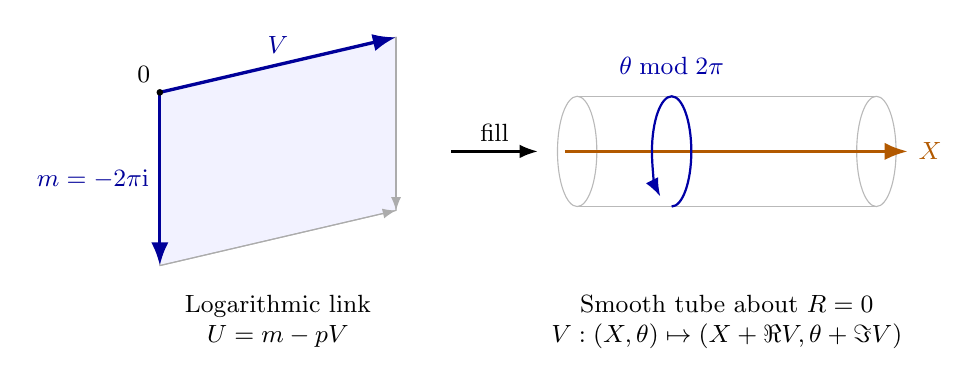
\begin{tikzpicture}[x=1cm,y=1cm,>=Latex,font=\small,
 period/.style={very thick,->,blue!60!black},
 boundary/.style={thin,gray!65}]
 \begin{scope}[shift={(0,0)}]
  \coordinate (o) at (0,1.8);
  \coordinate (m) at (0,-.4);
  \coordinate (v) at (3,2.5);
  \coordinate (mv) at (3,.3);
  \fill[blue!5] (o)--(v)--(mv)--(m)--cycle;
  \draw[boundary] (o)--(v)--(mv)--(m)--cycle;
  \draw[period] (o)--(m) node[midway,left] {$m=-2\pi\ii$};
  \draw[period] (o)--(v) node[midway,above] {$V$};
  \draw[->,gray!65] (m)--(mv);
  \draw[->,gray!65] (v)--(mv);
  \fill (o) circle (1.2pt);
  \node[above left] at (o) {$0$};
  \node[below,align=center] at (1.5,-.65)
       {Logarithmic link\\$U=m-pV$};
 \end{scope}
 \draw[->,thick] (3.7,1.05)--(4.8,1.05)
      node[midway,above] {fill};
 \begin{scope}[shift={(5.3,1.05)}]
  \draw[gray!55] (0,-.7)--(3.8,-.7);
  \draw[gray!55] (0,.7)--(3.8,.7);
  \draw[gray!55] (0,0) ellipse (.25 and .7);
  \draw[gray!55] (3.8,0) ellipse (.25 and .7);
  \draw[very thick,orange!70!black,->] (-.15,0)--(4.2,0)
      node[right] {$X$};
  \draw[blue!65!black,thick,->]
       (1.2,-.7) arc[start angle=-90,end angle=235,
                     x radius=.25,y radius=.7];
  \node[above,blue!65!black] at (1.2,.85) {$\theta\bmod 2\pi$};
  \node[below,align=center] at (1.9,-1.7)
      {Smooth tube about $R=0$\\
       $V:(X,\theta)\mapsto(X+\Re V,\theta+\Im V)$};
 \end{scope}
\end{tikzpicture}

\caption{The logarithmic link and its filling. The vertical period
\(m=U+pV=-2\pi\ii\) is the primitive meridian of the added solid torus;
the other displayed period is the original disk longitude \(V\).
The old basis is recovered by \(U=m-pV\). The tube coordinates
\((X,\theta)\) identify translation by \(V\) with a translation along
the axis together with a rotation, while \(m\) is one full angular
turn. The drawing uses a scaled vertical axis.}
\label{mf:filling-figure}
\end{figure}

The branch in Section~\ref{mf:critical} satisfies every hypothesis
of Proposition~\ref{mf:completion-prop}. It is an actual representation
in one bounded complete frame; the selected flags are holomorphic;
the main peripheral groups remain translations; and
\(\Rea V_e>0\). The exact slope equation is \(-2\pi\ii\).
This proves the metric assertion of Theorem~\ref{mf:main}, including
zero restrictions on relative signs or relative rates of the
independently long powers.

\section{The absolute action and the same filled fundamental chain}
\label{mf:regulator}

\subsection{The peripheral differential and its factor}

Fix the shape convention before computing a sign. We orient
upper half-space by \(dx\wedge dy_{\rm hor}\wedge dh\).
The positively ordered model is
\((a_0,a_1,a_2,a_3)=(0,\infty,1,z)\), with \(\Ima z>0\);
approximating infinity by height \(H\) gives determinant
\(H\Ima z>0\). For general vertices our cross-ratio is
\[
 z=\frac{(a_3-a_0)(a_2-a_1)}
          {(a_3-a_1)(a_2-a_0)}.
\]
Its signed volume is \(D(z)\). The outward cusp orientation at
infinity is the usual complex orientation. We take peripheral
bases of positive intersection in that orientation, as is the
rectangle basis with \(\Ima(\lambda/\mu)>0\).

Retain the positive ideal triangulation of the original exterior
constructed in Section~\ref{mf:topology}. Develop its ideal vertices
at the continued peripheral flags of the representation.
Their ordered cross-ratios remain positive near the complete point.
Every face and edge equation holds because the developed vertices
come from the same representation and the original group words.
Let \(\beta_\rho=\sum_\Delta[z_\Delta]\), with the original
orientations, be this fundamental ideal chain, and put
\(\mathcal V_\rho=\sum_\Delta D(z_\Delta)\).
Here the Bloch--Wigner volume is
\[
 D(z)=\Ima\operatorname{Li}_2(z)+\log|z|\,\arg(1-z),\qquad
 dD=\log|z|\,d\arg(1-z)-\log|1-z|\,d\arg z .
\]
The local logarithms are continued in this one positive shape chart.

We spell out the boundary normalization used below. For a positively
ordered tetrahedron use logarithms \(u=\log z\) and
\(v=\log(1-z^{-1})\), with symplectic form \(du\wedge dv\);
reverse the form for a reversed tetrahedron.
The three opposite-edge coordinate vectors are
\[
                 e_0=(1,0),\quad e_1=(0,1),\quad e_2=(-1,-1).
\]
The type of edge \(ij\) is \(0\) for \(01,23\), \(1\) for
\(02,13\), and \(2\) for \(03,12\); thus
\(\operatorname{type}(j,f)\) means the type of edge joining
vertices \(j,f\). Face \(f\) is opposite vertex \(f\).
Here is the geometric identification of the normal-path rows.
At each vertex send that vertex to infinity and normalize its first
two remaining vertices, in increasing order, to \(0,1\).
The third is respectively
\(z^{-1},z,(1-z^{-1})^{-1},(1-z)^{-1}\) for vertices \(0,1,2,3\).
The logarithms of the three opposite cusp-side vectors, in increasing
other-face order, are therefore, up to constant multiples of \(\pi\ii\),
\begin{equation}\label{mf:cusp-side-table}
\begin{array}{c|ccc}
 j&\ell_{f_0}&\ell_{f_1}&\ell_{f_2}\\ \hline
 0&v&-u&0\\
 1&u+v&u&0\\
 2&-u-v&-v&0\\
 3&-v&-u-v&0 .
\end{array}
\end{equation}
For instance at infinity, \(j=1\), the cusp triangle is \(0,1,z\)
and its sides have vectors \(z-1,z,1\).
If \(a_i\) is the scale taking the \(i\)-th canonical cusp triangle
into a common developed chart, a shared side gives
\(a_{i+1}/a_i=-\mathrm{side}_{\rm out}(i)/
\mathrm{side}_{\rm in}(i+1)\). Around a closed normal path the scales
telescope. Its actual similarity multiplier is the product of
outgoing sides divided by incoming sides, including the fixed signs.
Thus its logarithmic row is the sum of the outgoing-flow-weighted
entries of \eqref{mf:cusp-side-table}. The table proves that this row
is exactly the vector \(d_j(r)\) below, in the coordinates \((u,v)\).

The following local calculation records the intersection factor.
In tetrahedron orientation \(\varepsilon\),
at vertex \(j\) list the other faces \(f_0<f_1<f_2\).
A normal flow has outgoing entries \(r_{j,f}\) across the three sides
of that cusp triangle, with \(\sum_{f\ne j}r_{j,f}=0\).
In the next two formulas we suppress the first index within a fixed
vertex \(j\), writing \(r_{f_i}=r_{j,f_i}\).
Set
\[
 d_j(r)=(-1)^j\!
    \left(r_{f_1}e_{\operatorname{type}(j,f_2)}
              -r_{f_2}e_{\operatorname{type}(j,f_1)}\right),
 \qquad \tau_j=-\varepsilon(-1)^j .
\]
The oriented triangle intersection is
\(\frac12\tau_j(r_{f_0}s_{f_1}-r_{f_1}s_{f_0})\).
Expanding the two-coordinate determinants gives
\begin{equation}\label{mf:normal-flow}
 \Omega_\varepsilon(d(r),d(s))
 +\sum_j\tau_j(r_{f_0}s_{f_1}-r_{f_1}s_{f_0})
 =\sum_f\varepsilon(-1)^f r_f^{\mathsf t}
       \begin{pmatrix}0&1&-1\\-1&0&1\\1&-1&0\end{pmatrix}s_f .
\end{equation}
Here \(d=\sum_jd_j\), and the column \(r_f\) on the right lists
\((r_{j,f})_{j\ne f}\) in increasing vertex order, as does \(s_f\).
This identity is verified by substituting the three displayed vectors
and eliminating the third flow at each vertex. Each flow therefore
has eight independent variables; expanding all their bilinear
coefficients proves the identity.
The face terms cancel on glued faces: a permutation matrix \(P\)
conjugates the displayed skew matrix to \(\operatorname{sign}(P)\)
times itself. Thus peripheral rows pair by minus twice their
oriented intersection number. Distinct tori pair to zero.

For completeness, a small normal circle about an endpoint of a
global edge has vector equal, up to orientation, to that edge's
signed shape-incidence row: each successive corner contributes its
opposite-edge type. It is null-homologous in the cusp triangulation.
The same face cancellation in \eqref{mf:normal-flow} therefore makes
every edge row orthogonal to every closed peripheral row and to
every other such small edge circle. This proves edge isotropy.
Its only linear dependencies are the cusp-vertex ones. A dependency assigns numbers
\(\lambda_{ij}\) to the six edges of each tetrahedron whose opposite
sums are equal. It has the form
\(\lambda_{ij}=s_i+s_j\): solve for the four \(s_i\) from any
three incident pairs and the opposite-sum equations.
A face identifies the three \(s_i\) uniquely, so they descend exactly
to one value per ideal vertex. For \(t\) tetrahedra and \(c\) torus
cusps, the number of edges is \(t\), by Euler characteristic, hence
the edge rank is \(t-c\). The row quotient has dimension \(2c\).
Primitive peripheral rows form a basis because their pairings are
\(-2\) on each cusp and zero between cusps. To pass from rows to
tangent vectors, let
\(J=\bigoplus_\Delta\varepsilon_\Delta
\left(\begin{smallmatrix}0&1\\-1&0\end{smallmatrix}\right)\)
and let \(E\) be the edge-row span.
The edge-equation tangent space is the annihilator
\(W=\{X:aX=0\ (a\in E)\}\); its null directions are \(JE^{\mathsf t}\).
Peripheral rows annihilate these null directions.
If \(a,b\) are the meridian and longitude rows of one cusp, then
\(aJb^{\mathsf t}=-2\).
Modulo null directions their dual tangent vectors are
\(-Jb^{\mathsf t}/2\) and \(Ja^{\mathsf t}/2\).
Their \(J\)-pairing is \(-1/2\).
Cross-cusp pairings vanish, and the \(2c\) vectors exhaust the
quotient \(W/JE^{\mathsf t}\). Thus its tangent form is
\[
                   -\frac12\sum_i dU_i\wedge dV_i.
\]
In these shape coordinates,
\(dD=\Rea u\,d\Ima v-\Rea v\,d\Ima u\).
The real shape-log vector and the variation of its imaginary part
both lie in \(W\): the real edge sums are zero
and the imaginary edge sums are constant multiples of \(2\pi\).
Their peripheral coordinates are respectively
\((\Rea U,\Rea V)\) and \((d\Ima U,d\Ima V)\).
Applying the reduced pairing to these two vectors proves
\begin{equation}\label{mf:volume-differential}
 d\mathcal V_\rho
   =\frac12\sum_i
       \bigl(\Rea V_i\,d\Ima U_i-\Rea U_i\,d\Ima V_i\bigr).
\end{equation}
The fixed central signs in peripheral lifts have zero real part and
zero derivative, so centering their logarithms at completeness does
not alter this calculation. This supplies the factor for similarity
logs, rather than eigenvalue logs.
The classical peripheral-volume framework is discussed by
Neumann--Zagier~\cite{NeumannZagier}; the calculation above fixes the
present conventions component by component.

\subsection{Absolute calibration and the filling correction}

Equation \eqref{mf:action-peripheral} gives
\[
                d(2\pi\ii A_\epsilon)=-\tfrac12\sum_eU_e\,dV_e.
\]
Taking real and imaginary parts and using
\eqref{mf:volume-differential} shows that
\(2\pi\Rea A_\epsilon-\mathcal V_\rho
                       +\frac12\sum_e\Ima U_e\Rea V_e\)
is constant. It vanishes at completeness by
\eqref{mf:complete-volume}--\eqref{mf:Phi}. Hence
\begin{equation}\label{mf:absolute-regulator}
 2\pi\Rea A_\epsilon
       =\mathcal V_\rho-\frac12\sum_e\Ima U_e\,\Rea V_e.
\end{equation}
This uses the complete volume of the original polyhedra as the
constant. Agreement of derivatives or Hessians would not fix it.

At the critical point,
\(U_e=4\pi\ii p_e\delta_e-2\pi\ii\) and
\(V_e=-4\pi\ii\delta_e\). Directly,
\begin{equation}\label{mf:boundary-cancel}
 \Rea(-2\pi\ii p_e\delta_e^2+2\pi\ii\delta_e)
     =\frac1{4\pi}\Ima U_e\,\Rea V_e .
\end{equation}
Since \(S_{\mathbf n}=A_\epsilon+
\sum_e(-2\pi\ii p_e\delta_e^2+2\pi\ii\delta_e)\),
\eqref{mf:absolute-regulator} becomes \(2\pi\Rea S_{\mathbf n}
=\mathcal V_\rho\).

\subsection{Why this is the volume of the filled metric}

The last equality must use the same original fundamental class.
We give the comparison explicitly. For a peripheral map fixing an
axis, use a comparison map taking the end into that axis. After a
conjugation its endpoints are \(0,\infty\), and it has the form
\((0,Y e^{\chi(w)})\), where the character \(\chi\) is real-linear
on the peripheral cover. The original conical developing chain has
the form
\((a(w),Yb(w))\) on each boundary triangle; on a finite fundamental
set \(a,b\) and their derivatives are bounded and \(b>0\).
Use precisely that boundary triangulation for the homotopy
\begin{equation}\label{mf:boundary-homotopy}
 H_s(w,Y)=
 \left(sa(w),\,
       Y\exp\bigl((1-s)\chi(w)+s\log b(w)\bigr)\right),
 \qquad 0\le s\le1 .
\end{equation}
It is equivariant because both heights transform by the same positive
multiplier and the horizontal coordinate by the same complex
multiplier. On a fundamental boundary triangle the height is comparable
to \(Y\), horizontal derivatives are bounded, and height derivatives
are \(O(Y)\). Hyperbolic volume is \(y^{-3}\,dx\,dy_{\rm hor}\,dy\);
therefore the homotopy's three-dimensional volume is \(O(Y^{-2})\).
The same estimate applies to any subdivision and to the parabolic
conical comparison at a main cusp.

After filling, extend this \emph{same} axis-valued boundary
triangulation over the solid torus. The primitive slope has been
killed, so the extension is equivariant; the remaining cyclic group
acts by translation along the axis. Every added tetrahedron is
collinear and has zero signed volume. Stokes, first on finite
truncations and then as \(Y\to\infty\), now identifies the original
ideal-chain volume \(\mathcal V_\rho\) with the equivariant volume
of the filled representation. Replacing an unrelated new set of
vertices by axis points would not establish this equality.

Finally compare this equivariant chain with the developing map of
the complete metric from Proposition~\ref{mf:completion-prop}.
They represent the same filled fundamental class and agree at the
remaining cusp flags. Straightening their common finite subdivision
and applying the same vanishing boundary estimate gives
\(\mathcal V_\rho=\Vol\) of that metric.
This proves \eqref{mf:volume} for the constructed complete metric.
The usual hyperbolic volume is independent of a choice of complete
metric; the following short volume argument also establishes the
needed independence without a rigidity equality case.

\begin{lemma}\label{mf:volume-independence}
Two oriented complete finite-volume hyperbolic metrics on the same
marked cusped three-manifold have the same volume.
\end{lemma}
\begin{proof}
We recall the inequality needed for this conclusion.
For a complete source metric and a boundary-parabolic representation,
choose an equivariant map, affine-conical on its cusps.
It is globally Lipschitz after a compact-core smoothing.
Smear a finite regular hyperbolic tetrahedron \(T_R\) over the
oriented isometry quotient, with Haar measure normalized by the
source volume. Fubini gives the integral of its pulled-back volume
as
\(\Vol(T_R)\Vol(\rho)/\Vol(M)\).
Straighten the four image vertices. The difference is the sum of
the four face-homotopy prisms. Their integrals cancel in pairs:
the ordered faces of a regular tetrahedron are congruent, Haar
measure is invariant, and their boundary signs alternate.
The Lipschitz bound on fixed finite \(T_R\) justifies these finite
integrals; cusp truncations give the same formula by the preceding
boundary estimate.

Every straight tetrahedron has absolute volume at most the regular
ideal volume \(v_3\). In the Klein ball enlarge its vertex rays to
the ideal boundary; an oriented nondegenerate tetrahedron's unsigned
volume increases. For an ideal tetrahedron the Lobachevsky formula is
\(\Lambda(\alpha)+\Lambda(\beta)+\Lambda(\gamma)\), with
\(\alpha+\beta+\gamma=\pi\). It vanishes on the boundary.
An interior critical point has
\(\sin\alpha=\sin\beta=\sin\gamma\), hence
\(\alpha=\beta=\gamma=\pi/3\). Its maximum is therefore \(v_3\).
Thus
\[
        |\Vol(\rho)|\le
             \frac{v_3}{\Vol(T_R)}\Vol(M).
\]
Let \(R\to\infty\). Apply the resulting inequality to the holonomy
of each metric with the other as source. Its equivariant volume is
its metric volume by the same fundamental-chain comparison.
The two opposite inequalities prove equality.
\end{proof}

\section{The interface with source asymptotics}
\label{mf:interface}

Theorem~\ref{mf:main} has only classical inputs: the labeled matched
sphere, the original disk paths, and the independently long fixed
integer fillings. In particular, the functions \(Q_b,A_0,S_{\mathbf n}\)
were defined here by angles, not by a limit of polynomials.
If a finite source calculation produces these same local functions
and the original primitive framing, it may use the following precise
output.

\begin{corollary}[Geometric identification of a selected action]
\label{mf:interface-cor}
Suppose a separately proved source theorem for the specified original
diagram has the action \eqref{mf:filling-action}, with its roots and
logarithms continued from the complete face-critical point.
For fixed independently sufficiently long signed powers, its
unit-charge critical point is the classical point of
Section~\ref{mf:critical}. Its real limiting action is
\(\Vol(S^3\setminus K_{\mathbf p})/(2\pi)\) when the original
component test is a knot, and the corresponding filled link volume
otherwise.
\end{corollary}
\begin{proof}
The source equations and this paper's equations are identical in
the specified germ. The implicit-function uniqueness in
Section~\ref{mf:critical} identifies their critical points.
Theorem~\ref{mf:main} then gives the claim.
\end{proof}

The companion oscillatory filling theorem
\cite[Theorem 1.1]{OscillatoryFillings} requires a nonzero uniform
local packet and a strict complementary strip bound for the
\emph{actual finite polynomial}. The present paper neither assumes
nor proves those analytic hypotheses. It also gives no comparison
between central and one-sided crossing sectors. To deduce a full
invariant limit, the finite diagram identity, all parity and framing
factors, noncancellation of the whole central period, and a bound on
the remaining original sectors must be supplied separately.
The geometric conclusion identifies their volume target when those
inputs have been proved; it does not replace them.

\begin{thebibliography}{9}
\bibitem{BobenkoSpringborn}
A.~I. Bobenko and B.~A. Springborn,
\emph{Variational principles for circle patterns and Koebe's theorem},
Trans. Amer. Math. Soc. \textbf{356} (2004), 659--689.
\href{https://arxiv.org/abs/math/0203250}{arXiv:math/0203250}.

\bibitem{Lee}
J.~M. Lee, \emph{Introduction to Smooth Manifolds}, second edition,
Graduate Texts in Mathematics 218, Springer, 2013.
\href{https://doi.org/10.1007/978-1-4419-9982-5}
{doi:10.1007/978-1-4419-9982-5}.

\bibitem{Milnor}
J.~Milnor, \emph{Hyperbolic geometry: the first 150 years},
Bull. Amer. Math. Soc. (N.S.) \textbf{6} (1982), 9--24.
\href{https://doi.org/10.1090/S0273-0979-1982-14958-8}
{doi:10.1090/S0273-0979-1982-14958-8}.

\bibitem{NeumannZagier}
W.~D. Neumann and D.~Zagier,
\emph{Volumes of hyperbolic three-manifolds},
Topology \textbf{24} (1985), 307--332.
\href{https://doi.org/10.1016/0040-9383(85)90004-7}
{doi:10.1016/0040-9383(85)90004-7}.

\bibitem{Rivin}
I.~Rivin, \emph{Euclidean structures on simplicial surfaces and
hyperbolic volume}, Ann. of Math. (2) \textbf{139} (1994), 553--580.
\href{https://doi.org/10.2307/2118572}{doi:10.2307/2118572}.

\bibitem{OscillatoryFillings}
\emph{Oscillatory filling sums with independently long twists},
companion paper, Theorem 1.1.
\url{https://sashakolpakov.github.io/murakamis_dream/papers/oscillatory-fillings.pdf}.
\end{thebibliography}
\end{document}
